\documentclass[10pt,a4paper]{article}
\usepackage[utf8]{inputenc}
\usepackage[francais]{babel}
\usepackage{color}
\usepackage[T1]{fontenc}
\usepackage{amsmath}
\usepackage{amsfonts}
\usepackage{amssymb}
\usepackage{graphicx}
\usepackage{hyperref}
\usepackage[margin=3cm]{geometry}
\newcommand{\ssi}{\textit{ssi. }}
\renewcommand{\mod}{\text{ mod }}
\author{Guillaume \textsc{Huysmans} et Florent \textsc{Delgrange}}
\title{Intelligence Artificielle\\Pré-projet}
\date{30 mars 2016}
\begin{document}
\maketitle
\section{Introduction}
Il nous a été demandé d'implémenter 3 IA pour le jeu de Nim :
\begin{enumerate}
\item Une IA aléatoire qui gagne en un tour si elle en a la possibilité et joue
	aléatoirement sinon.
\item Une IA qui joue de manière optimale à chaque tour <<~si possible~>>
	(nous reviendrons sur cette notion plus tard) et aléatoirement sinon.
\item Une IA coopérative qui permet de jouer à deux contre un.
\end{enumerate}

Ce rapport expliquera les algorithmes que nous avons développés
pour résoudre ces problèmes.

\section{IA aléatoire améliorée}
L'IA joue aléatoirement jusqu'à ce qu'il soit possible pour elle de faire un
coup gagnant. Un coup gagnant correspond au moment dans le jeu où il reste, au
plus, autant de pions que le nombre de pions qu'on a le droit de déplacer.

Soient $m$, le nombre de pions restant et $n$ le nombre de pions maximum qu'on
est autorisé à déplacer. Nous nous trouvons dans une situation gagnante \ssi
\[m \mod (n+1) = m \Leftrightarrow m \leq n\]

Notre IA joue aléatoirement jusqu'à atteindre cet objectif.
Dès que c'est le cas, elle retire $n$~pions et gagne la partie.

\section{IA gagnante}
Soient $m$, le nombre de pions restants et $n$ le nombre de pions maximum qu'on
est autorisé à déplacer. Un coup est dit optimal \ssi à chaque tour,
celui-ci correspond à $m \mod (n+1)$ à condition que $m \mod (n+1) \neq 0$.
Dans le cas contraire, l'IA ne sait pas jouer de manière optimale et joue
aléatoirement.
Afin d'illustrer cette propriété, nous allons utiliser un
graphe que nous avons généré par programme.
\begin{figure}
\makebox[\textwidth][c]{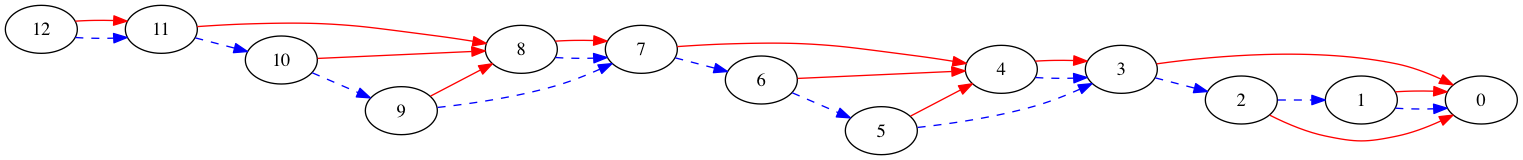
\includegraphics[width=1.2\textwidth]{nim.png}}
\caption{Déroulement d'un jeu de Nim}
\label{nim12}
\end{figure}

La figure~\ref{nim12} représente l'évolution d'un jeu de Nim avec $m=12$ et
$n=3$. Nous considérons pour cet exemple, par souci de lisibilité, que lorsque
l'IA ne peut pas jouer de coup gagnant, elle ne retire qu'un pion au lieu de
jouer aléatoirement. Le parcours correspondant à cette IA est décrit par le
chemin tracé en {\color{red} rouge} (trait plein).
Les sommets de ce graphe représentent le
nombre de pions restants et les arcs, le nombre de pions que l'IA retire.

L'IA gagnante va donc <<~bloquer~>> l'adversaire à chaque tour, l'empêchant
d'arriver au cas où $m \mod (n+1) = m$ (le cas où il reste au plus autant de
jetons que de jetons maximum qu'il est possible de retirer). Lorsque l'IA
gagnante tombe dans ce cas de base, elle gagne.

Ce ne sera pas toujours possible puisque dans le cas trivial (dans l'exemple)
où elle commence avec 4 jetons, elle pourra en laisser entre 1 et 3
à son adversaire qui gagnera dans tous les cas.

\section{IA coopérative}
Deux joueurs ligués doivent être sûrs de gagner c'est-à-dire que le joueur 1 ou
le joueur 2 doit gagner la partie. Cette IA a pour but de permettre au joueur
qui joue au tour suivant de toujours avoir la possibilité de faire un coup
optimal. Soient $m$, le nombre de pions restants et n le nombre de pions maximum
qu'on est autorisé à déplacer. L'IA permet au joueur suivant de faire un coup
optimal (comme défini à la section précédente) \ssi l'IA retire $x$
jetons, $x$ étant défini de la façon suivante :
\begin{align}
	x &\in [1, min(n, m)] &&
	\text{si } m \mod (n+1) = 0 \text{ ou } m \mod (n+1) = n \label{s1} \\
	x &= 2 && \text{si } (m-1) \mod (n+1) = 0 \label{s2} \\
	x &= 1 && \text{sinon} \label{s3}
\end{align}

Pour illustrer cette propriété, nous nous référons à nouveau à la figure
~\ref{nim12}. Le parcours correspondant à cette IA est décrit par le chemin
tracé en {\color{blue} bleu} (trait discontinu).

Dans le cas \eqref{s1}, par le fait que
$m \mod (n+1)=0$, n'importe quel coup porté par le joueur jouant au tour
suivant aura la possibilité d'être optimal. De plus, si $m \mod (n+1) = m$, alors
on peut également jouer aléatoirement car cela signifie qu'il reste au plus $n$
pions et donc que l'IA coopérative permet soit au joueur suivant de gagner, soit
gagne en retirant le nombre de pions restants.

Le cas \eqref{s2}, correspond au cas où, si l'IA retire 1 jeton, celle-ci bloque
le joueur suivant et lui interdit de jouer de manière optimale.
L'IA retire alors 2~jetons pour assurer au joueur suivant la possibilité de
placer un coup optimal.

Finalement, le cas \eqref{s3} ne nous
permet pas de jouer aléatoirement dans $[1, n]$ car on pourrait encore une fois
bloquer le joueur suivant. Cependant, il est tout à fait possible de retirer un
jeton pour garantir au joueur suivant de jouer de manière optimale.

Il est donc trivial que son association avec l'IA gagnante lui garantira
la victoire lors de parties de 3 joueurs avec $n \geq 2$.  En effet,
l'IA coopérative permettra à chaque tour à l'IA gagnante de bloquer
l'adversaire.

\section{Remarque}
Nous aurions voulu ne créer qu'une seule IA capable de décider d'aider le joueur
suivant si il est dans son équipe ou d'attaquer celui-ci dans le cas où c'est
un adversaire, mais le framework ne permet malheureusement
pas à un joueur de déterminer qui joue avec lui.

\section{Conclusion}
Le jeu tel qu'il nous a été présenté est donc totalement résolu;
on peut sous certaines conditions garantir la victoire d'un des joueurs.
Le premier joueur ne gagnera pas forcément,
cela dépend du nombre initial de jetons.

\end{document}
